% Cartly engineering report. Build: see README.md in this folder.
\documentclass[11pt,a4paper]{report}

\usepackage{fontspec}
\setmainfont{texgyreheros}[Extension=.otf,UprightFont=*-regular,BoldFont=*-bold,ItalicFont=*-italic,BoldItalicFont=*-bolditalic]
\setmonofont{texgyrecursor}[Extension=.otf,UprightFont=*-regular,BoldFont=*-bold,ItalicFont=*-italic,BoldItalicFont=*-bolditalic,Scale=0.88]
\usepackage[a4paper,margin=2.6cm,headheight=14pt]{geometry}
\usepackage{microtype}
\usepackage{setspace}
\setstretch{1.12}
\usepackage{parskip}
\setlength{\parskip}{0.55em}
\usepackage{amsmath}
\usepackage{xcolor}
\usepackage{booktabs,tabularx,array,longtable}
\usepackage{enumitem}
\setlist{nosep,leftmargin=1.4em,itemsep=0.25em}
\usepackage{caption}
\captionsetup{font=small,labelfont=bf,skip=6pt}
\usepackage{float}
\usepackage{titlesec}
\usepackage{fancyhdr}
\usepackage{listings}
\usepackage{tikz}
\usetikzlibrary{arrows.meta,positioning,shapes.geometric,fit,calc,backgrounds}
\usepackage[hidelinks,pdfusetitle]{hyperref}

% Semantic colours only (information / success / warning / risk). Everything else is black on white.
\definecolor{info}{HTML}{1F5FA8}
\definecolor{ok}{HTML}{23703A}
\definecolor{warn}{HTML}{9A6200}
\definecolor{risk}{HTML}{A82B2B}
\definecolor{rule}{HTML}{BBBBBB}
\definecolor{paper}{HTML}{F4F4F4}

\titleformat{\chapter}[hang]{\bfseries\LARGE}{\thechapter}{0.8em}{}[\vspace{2pt}\titlerule]
\titlespacing*{\chapter}{0pt}{-10pt}{18pt}
\titleformat{\section}{\bfseries\Large}{\thesection}{0.7em}{}
\titleformat{\subsection}{\bfseries\large}{\thesubsection}{0.6em}{}
\titlespacing*{\section}{0pt}{16pt}{6pt}
\titlespacing*{\subsection}{0pt}{12pt}{4pt}

\pagestyle{fancy}
\fancyhf{}
\fancyhead[L]{\small Cartly: engineering report}
\fancyhead[R]{\small\leftmark}
\fancyfoot[C]{\small\thepage}
\renewcommand{\headrulewidth}{0.3pt}
\renewcommand{\chaptermark}[1]{\markboth{#1}{}}

\lstset{
  basicstyle=\ttfamily\footnotesize,
  backgroundcolor=\color{paper},
  frame=single, rulecolor=\color{rule},
  breaklines=true, columns=fullflexible, keepspaces=true,
  xleftmargin=0.3em, xrightmargin=0.3em, aboveskip=8pt, belowskip=6pt,
  showstringspaces=false
}

% Inline helpers
\newcommand{\code}[1]{\texttt{\small #1}}
\newcommand{\tagimpl}{\textcolor{ok}{\textbf{Implemented}}}
\newcommand{\tagtest}{\textcolor{info}{\textbf{Tested}}}
\newcommand{\tagplan}{\textcolor{warn}{\textbf{Not built}}}
\newcommand{\tagunver}{\textcolor{risk}{\textbf{Not verified}}}

% Callout (restrained: a rule on the left, no fill colour)
\newcommand{\callout}[2]{%
  \par\noindent\begin{minipage}{\dimexpr\linewidth}%
  \noindent\rule{0.6pt}{0pt}\hspace{-0.6pt}%
  \begin{tabular}{@{}|@{\hspace{8pt}}p{0.93\linewidth}@{}}
  \textbf{#1}\newline #2
  \end{tabular}%
  \end{minipage}\par\vspace{4pt}}

% TikZ styles
\tikzset{
  box/.style={draw, rectangle, minimum height=7mm, align=center, font=\small, inner sep=4pt},
  mod/.style={box, fill=paper},
  ext/.style={box, dashed},
  store/.style={box, fill=paper, rounded corners=1pt},
  arr/.style={-{Stealth[length=2.2mm]}, thick},
  darr/.style={-{Stealth[length=2.2mm]}, thick, dashed},
  lbl/.style={font=\scriptsize, midway, fill=white, inner sep=1.5pt}
}

\begin{document}
\begin{titlepage}
\thispagestyle{empty}
\vspace*{3.2cm}
{\Huge\bfseries Cartly}\par
\vspace{6pt}
{\LARGE An Engineering Reconstruction of a\\Marketplace-Scale Shopping Experience}\par
\vspace{14pt}
\rule{\linewidth}{0.6pt}\par
\vspace{6pt}
{\large Amazon.com Clone --- 24-Hour Software Engineering Challenge}\par
{\large Engineering Report}\par
\vspace{2.2cm}

\begin{tabular}{@{}p{3.4cm}p{10.5cm}@{}}
\textbf{Author} & Nitish R.G. \\[3pt]
\textbf{Date} & 3 October 2026 \\[3pt]
\textbf{Repository} & \code{github.com/NITISH-R-G/amazon-clone} (branch \code{main}) \\[3pt]
\textbf{Deployment} & \code{amazon-clone-six-sigma-27.vercel.app} (Vercel, HTTPS) \\[3pt]
\textbf{Stack} & Next.js 16, React 19, TypeScript (strict), PostgreSQL with Drizzle ORM, Stripe (test mode), Vitest, Playwright \\[3pt]
\textbf{Scope} & A fictional marketplace: invented brands, sellers, products and reviews. No Amazon data or assets are used. \\
\end{tabular}

\vfill
{\small\textbf{Reading guide.} Throughout this report, claims are labelled by their evidence:
\tagimpl{} (present in the source), \tagtest{} (covered by an automated test), \tagplan{} (considered or designed only) and
\tagunver{} (could not be confirmed from the repository).}
\end{titlepage}

\tableofcontents
\listoffigures
\listoftables

\chapter*{Executive Summary}
\addcontentsline{toc}{chapter}{Executive Summary}
\markboth{Executive Summary}{}

\textbf{The challenge.} Rebuild the Amazon.com shopping experience in roughly 24 hours (the repository history spans about 22 hours, from the first commit on 2 October to the last on 3 October 2026), and be judged on speed, product judgment and UX quality.

\textbf{The objective we set.} Do not produce a visual clone. The visible interface of a marketplace is the surface of a stateful system: a catalogue with typed attributes, variants that carry their own price and stock, competing seller offers, reservations that stop two customers buying the same last unit, a payment lifecycle that is separate from the order lifecycle, and ranking rules that decide what each customer sees. We built a small version of that system and made every customer-visible number (price, discount, delivery date, rating) a server-side computation.

\textbf{What exists.} A Next.js application organised as a modular monolith (nine modules with enforced boundaries) on PostgreSQL, with a 2,400-product synthetic catalogue, multi-dimension variants, 608 additional seller offers on top of an implicit first-party offer, a deterministic buy-box rule, PostgreSQL full-text and trigram search with structured facets, a concept-based hybrid retrieval layer, a two-phase checkout with stock reservations, Stripe test-mode integration behind a provider interface (PaymentIntent, Payment Element, signed webhook), server-side coupons, a deterministic delivery promise, recently-viewed and deterministic recommendations, labelled sponsored placements, and verified reviews.

\textbf{What is verified.} 131 unit and integration tests across 26 files pass; type checking and linting are clean; Playwright journeys cover desktop and a phone viewport, including a two-browser race for the last unit of stock. The application is deployed over HTTPS on Vercel, and the final commits are recorded as successful production deployments.

\textbf{What is not verified.} A completed card payment against the live Stripe API was not performed from this repository's evidence; Stripe behaviour is covered by unit tests with real signature verification, and a key-gated end-to-end test exists but was not run. The database host in production is configured through an environment variable and is not independently confirmed here.

\begin{table}[H]
\centering
\caption{The project at a glance (all figures from the repository).}
\label{tab:glance}
\small
\begin{tabular}{@{}lr@{\qquad}lr@{}}
\toprule
Products & 2,400 & Database tables & 21 \\
Product types & 43 & SQL migrations & 20 \\
Fictional brands & 104 & Documented decisions & 32 \\
Variants & 8,860 & Unit/integration tests & 131 (26 files) \\
Seller offers & 608 & E2E scenarios & 12 $\times$ 2 viewports \\
Application modules & 9 & Source under \code{src/} & $\approx$13,900 lines \\
\bottomrule
\end{tabular}
\end{table}

\textbf{Main decisions.} PostgreSQL for everything, including search (no dedicated search engine); deterministic ranking everywhere (no machine learning); a payment-provider interface with a demo and a Stripe implementation; reservation-based inventory; and a hard rule that client-supplied prices, discounts and ``payment succeeded'' signals are never trusted.

\textbf{Main constraints.} Twenty-four hours; no access to real Amazon data; no paid external services beyond Stripe's free test mode. These drove the choices in Chapters~\ref{ch:scope} and~\ref{ch:decisions}.

\chapter{Problem Definition}
\label{ch:problem}

A basic storefront shows products, takes an order and sends an email. A marketplace like Amazon.com is a different kind of system, because almost every thing a customer sees is the output of a separate decision that must remain consistent with the others.

\begin{table}[H]
\centering
\caption{What a customer sees versus what must be true behind it.}
\label{tab:surface}
\small
\begin{tabularx}{\linewidth}{@{}lX@{}}
\toprule
On the page & Behind it \\
\midrule
A product with options & A \emph{product} (the idea), \emph{variants} (the exact purchasable configurations with their own SKU, price and stock) and \emph{offers} (who sells that variant, at what price, from where). \\
``In stock'' & A quantity that other customers are changing at the same moment, and that must not be sold twice. \\
A price & A seller's price, a list price, a deal, a coupon, shipping rules and tax, all computed in one agreed order. \\
Search results & Text matching, typo tolerance, structured filters whose options depend on the kind of product, and a ranking. \\
``Arrives Tue, Oct 6'' & A promise derived from fulfilment, handling time, cut-off and destination. \\
``Place order'' & A payment lifecycle (pending, failed, succeeded, refunded) that is not the same thing as the order lifecycle (awaiting payment, placed, shipped, delivered, cancelled). \\
Stars and reviews & Aggregates that must match the review records, and a ``verified purchase'' flag that must mean something. \\
\bottomrule
\end{tabularx}
\end{table}

The central engineering thesis of this project follows from the table: \emph{the visible shopping interface is only the surface of a much larger stateful marketplace system}. A visual copy of the pages would show none of the hard parts. We therefore chose to reproduce the hard parts at small scale and to be explicit about where our rules are our own rather than Amazon's.

\chapter{Product Scope and Product Judgment}
\label{ch:scope}

With 24 hours, the question was never ``what can we build'' but ``what must be true for a reviewer to believe this is a marketplace, and what can we leave out without losing that belief''. Table~\ref{tab:scope} records the answer. The ordering of work followed one rule from the project's instructions: protect the purchase path (browse, variant, cart, checkout, order) first, and cut decoration before correctness.

\begin{table}[H]
\centering
\caption{Scope decisions: what was built, why, and what was deliberately deferred.}
\label{tab:scope}
\footnotesize
\begin{tabularx}{\linewidth}{@{}p{2.4cm}XXX@{}}
\toprule
Area & Implemented & Why it mattered & Deliberately deferred \\
\midrule
Catalogue & 2,400 synthetic products, 43 types with typed attributes, 104 invented brands & Scale and heterogeneity make search, facets and pagination real & Real product data and imagery (none was licensed) \\
Variants & Up to three dimensions, SKU per variant, price/stock/picture per variant & Variant identity is the core of ``a product page'' & Bundles, subscriptions \\
Sellers and buy box & 608 seller offers, implicit first-party offer, deterministic selection rule & Shows that one product can have several sellers & Seller dashboards, seller ratings, onboarding \\
Search & PostgreSQL full-text and trigram, facets, typo tolerance, concept-based hybrid layer & Discovery is how customers find anything & Dedicated search engine, learned ranking \\
Inventory & Time-limited reservations with row locking and a concurrency test & Overselling is the classic marketplace failure & Warehouses, multi-location stock \\
Checkout and payments & Two-phase checkout, Stripe test mode behind a provider interface, idempotent webhooks, refunds & Trust: money must follow verified facts & Saved cards, live payments, fraud checks \\
Pricing & Deals, server-side coupons, shipping and tax rules & Totals must be explainable and tamper-proof & A general promotion engine \\
Delivery & Deterministic delivery windows on product, cart, checkout and order & ``When will it arrive'' drives purchase decisions & Carrier integration, tracking \\
Discovery & Recently viewed, deterministic recommendations, personalised home rails, sponsored placements & Makes the home page react to the customer & Machine-learned recommendation, ad auction \\
Reviews & Reviews with a verified-purchase flag derived from delivered orders & Trust signal with real semantics & Votes, images, moderation \\
Accounts & Register, sign in, guest cart merge, order history; guest checkout stays open & Accounts should add history, not gate purchase & OAuth, saved addresses, returns \\
\bottomrule
\end{tabularx}
\end{table}

Deferred items are not failures; each was weighed against its cost in the time box and against whether its absence would change what a reviewer could verify. The recorded reasoning is in the project's decision log (D1--D32).

\chapter{System Architecture}
\label{ch:architecture}

\section{A modular monolith}

The application is one deployable Next.js program organised into modules. Each module exposes a small public interface (\code{index.ts}) and keeps its implementation in an \code{internal/} directory; a lint rule forbids importing another module's internals. This gives most of the design discipline of services without the operational cost, which suited a one-person, one-day build. \tagimpl{}

\begin{figure}[H]
\centering
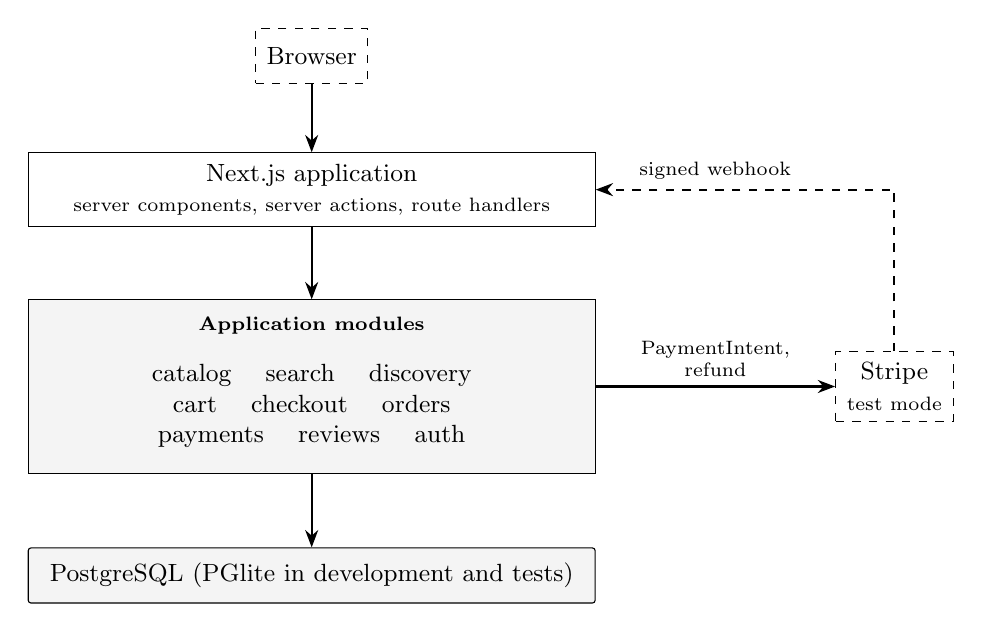
\begin{tikzpicture}
\node[ext] (browser) at (0,0) {Browser};
\node[box, minimum width=7.2cm] (next) at (0,-1.7) {Next.js application\\\scriptsize server components, server actions, route handlers};
\node[mod, minimum width=7.2cm, minimum height=2.2cm] (mods) at (0,-4.2) {};
\node[font=\scriptsize\bfseries, anchor=north] at ([yshift=-1mm]mods.north) {Application modules};
\node[font=\small, align=center] at ([yshift=-2.5mm]mods.center) {catalog \quad search \quad discovery\\cart \quad checkout \quad orders\\payments \quad reviews \quad auth};
\node[store, minimum width=7.2cm] (db) at (0,-6.6) {PostgreSQL (PGlite in development and tests)};
\node[ext] (stripe) at (7.4,-4.2) {Stripe\\\scriptsize test mode};
\draw[arr] (browser) -- (next);
\draw[arr] (next) -- (mods);
\draw[arr] (mods) -- (db);
\draw[arr] (mods.east) -- node[above, font=\scriptsize, align=center]{PaymentIntent,\\refund} (stripe.west);
\draw[darr] (stripe.north) |- node[pos=0.8, above, font=\scriptsize]{signed webhook} (next.east);
\end{tikzpicture}
\caption{Runtime view. Dashed boxes are external to the application.}
\label{fig:arch}
\end{figure}

\section{Module dependencies}

Figure~\ref{fig:deps} shows who may call whom. Checkout is the only orchestrator: it asks the cart for lines, the catalogue to reserve stock, payments to talk to the provider and orders to persist the result. The composition root (\code{src/server/app.ts}) is the only file that wires modules together.

\begin{figure}[H]
\centering
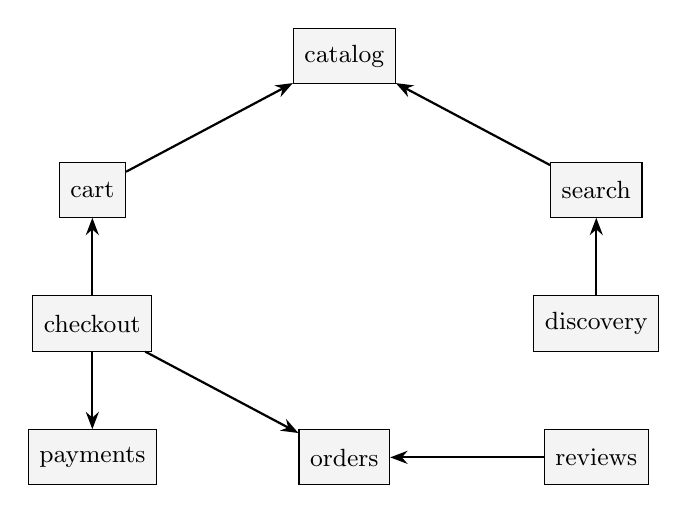
\begin{tikzpicture}
\node[mod] (catalog) at (3.6,0) {catalog};
\node[mod] (cart) at (0.4,-1.7) {cart};
\node[mod] (search) at (6.8,-1.7) {search};
\node[mod] (checkout) at (0.4,-3.4) {checkout};
\node[mod] (discovery) at (6.8,-3.4) {discovery};
\node[mod] (payments) at (0.4,-5.1) {payments};
\node[mod] (orders) at (3.6,-5.1) {orders};
\node[mod] (reviews) at (6.8,-5.1) {reviews};
\draw[arr] (cart) -- (catalog);
\draw[arr] (search) -- (catalog);
\draw[arr] (discovery) -- (search);
\draw[arr] (checkout) -- (cart);
\draw[arr] (checkout) -- (payments);
\draw[arr] (checkout) -- (orders);
\draw[arr] (reviews) -- (orders);
\end{tikzpicture}
\caption{Main module dependencies (arrow: ``uses''). Not drawn, to keep it readable: checkout, discovery and reviews also read the catalogue, and the route layer uses auth for sessions.}
\label{fig:deps}
\end{figure}

\section{Boundaries that make it testable}

Only three things are replaced by test doubles: the \emph{clock}, the \emph{identifier generator} and the \emph{payment provider}. The database is always real: tests run a genuine PostgreSQL engine in-process (PGlite), with the same migrations as production. This is deliberate. The interesting failures in this system (a lock that does not serialise, a constraint that does not hold) disappear if the database is mocked. \tagimpl{} \tagtest{}

\section{Technology stack}

\begin{table}[H]
\centering
\caption{Technologies actually used.}
\label{tab:stack}
\small
\begin{tabularx}{\linewidth}{@{}p{3.2cm}p{4.8cm}X@{}}
\toprule
Technology & Role & Reason \\
\midrule
Next.js 16 (App Router) & Routes, server rendering, server actions, route handlers & One deployable unit; server components keep pricing and ranking on the server \\
React 19, TypeScript (strict) & UI and types across the whole codebase & Types carry the domain model (money is integer cents) \\
Tailwind CSS 4, shadcn/ui, Radix & Components and styling & Accessible primitives; restrained monochrome design \\
PostgreSQL & System of record \emph{and} search engine & Transactions, row locks, full-text, trigram; one database to operate \\
Drizzle ORM & Schema and typed queries, SQL migrations & Schema in TypeScript; plain SQL where needed \\
PGlite & PostgreSQL in-process for development and tests & Fast, real engine; same SQL as production \\
\code{pg} & Production driver & Pooled connections to managed PostgreSQL \\
Stripe (SDK, Payment Element) & Test-mode payments & Real PaymentIntent lifecycle and signed webhooks \\
Zod & Input validation at boundaries & Shared parse-then-trust pattern \\
Vitest, Playwright & Unit/integration and end-to-end tests & Real database in tests; desktop and phone viewports \\
Vercel & Hosting over HTTPS & Git-connected deployment; migrations run at build time \\
pnpm, ESLint & Tooling & Reproducible installs; module-boundary lint rule \\
\bottomrule
\end{tabularx}
\end{table}

\section{Domain model}

The most important idea in the model is the three-level distinction between product, variant and offer (Figure~\ref{fig:pvo}). A \emph{product} is what a customer thinks of as ``the laptop''. A \emph{variant} is one exact configuration of it with its own SKU. An \emph{offer} is a particular seller's way of selling that exact variant. As an illustration (not a claim about a seeded item): the product ``Laptop X'' has the variant ``16~GB / 512~GB / Silver'', and ``Seller A'' may offer that variant at a given price and shipping cost while another seller offers the same variant for less but ships later.

\begin{figure}[H]
\centering
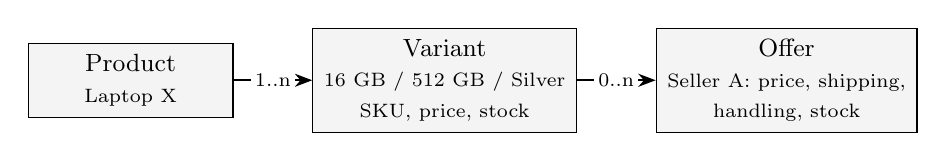
\begin{tikzpicture}[node distance=10mm]
\node[mod, minimum width=2.6cm] (p) {Product\\\scriptsize Laptop X};
\node[mod, right=of p, minimum width=3.2cm] (v) {Variant\\\scriptsize 16 GB / 512 GB / Silver\\\scriptsize SKU, price, stock};
\node[mod, right=of v, minimum width=3.2cm] (o) {Offer\\\scriptsize Seller A: price, shipping,\\\scriptsize handling, stock};
\draw[arr] (p) -- node[lbl]{1..n} (v);
\draw[arr] (v) -- node[lbl]{0..n} (o);
\end{tikzpicture}
\caption{Product, variant and offer. The variant row itself acts as the implicit first-party offer; seller offers are additional rows.}
\label{fig:pvo}
\end{figure}

Figure~\ref{fig:er} shows the main tables (21 in total; satellite tables such as sessions and campaigns omitted for readability).

\begin{figure}[H]
\centering
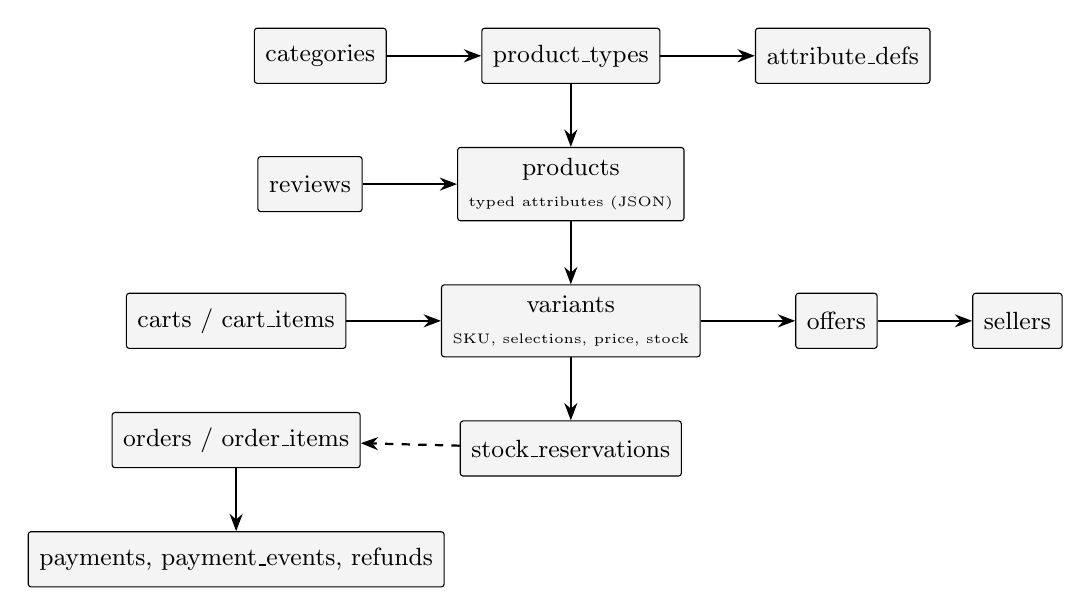
\begin{tikzpicture}[node distance=8mm and 12mm, every node/.style={font=\scriptsize}]
\node[store] (cat) {categories};
\node[store, right=of cat] (type) {product\_types};
\node[store, right=of type] (attr) {attribute\_defs};
\node[store, below=of type] (prod) {products\\\tiny typed attributes (JSON)};
\node[store, below=of prod] (var) {variants\\\tiny SKU, selections, price, stock};
\node[store, right=of var] (off) {offers};
\node[store, right=of off] (sel) {sellers};
\node[store, below=of var] (res) {stock\_reservations};
\node[store, left=of var] (cart) {carts / cart\_items};
\node[store, below=of cart] (ord) {orders / order\_items};
\node[store, below=of ord] (pay) {payments, payment\_events, refunds};
\node[store, left=of prod] (rev) {reviews};
\draw[arr] (cat) -- (type);
\draw[arr] (type) -- (attr);
\draw[arr] (type) -- (prod);
\draw[arr] (prod) -- (var);
\draw[arr] (var) -- (off);
\draw[arr] (off) -- (sel);
\draw[arr] (var) -- (res);
\draw[arr] (cart) -- (var);
\draw[arr] (ord) -- (pay);
\draw[arr] (rev) -- (prod);
\draw[darr] (res) -- (ord);
\end{tikzpicture}
\caption{Simplified entity relationships. Solid arrows: references. Dashed: reservation belongs to an order by identifier.}
\label{fig:er}
\end{figure}

Other tables: \code{promotions} (coupons), \code{product\_views}, \code{sponsored\_campaigns}, \code{users} and \code{sessions}. Money is stored as integer cents throughout, and order lines are purchase-time snapshots (title, price, SKU, seller) so that later catalogue changes never rewrite history.

\chapter{Catalogue, Variants and Marketplace}
\label{ch:catalogue}

\section{Catalogue and product model}

The seeded catalogue has 2,400 products: 30 hand-written (they carry the featured placements) and 2,370 generated deterministically from a seeded pseudo-random generator, so every environment gets the same data. They belong to 43 product types across nine departments, and carry 104 invented brand names. All pictures are flat illustrations generated by a script in the repository. \tagimpl{}

Products are not uniform records. Each \emph{product type} owns a set of \emph{attribute definitions}, each marked as a \emph{variation} attribute (what variants differ by: colour, storage, RAM) or a \emph{spec} attribute (a technical detail: refresh rate, processor), and optionally as a filter facet. A smartphone therefore has storage and RAM; a running shoe has size, colour, cushioning and terrain. A product stores its spec values as typed JSON keyed by attribute; the type supplies the vocabulary and labels. This lets the product page render a technical table and the search page offer the right filters without special-casing categories. \tagimpl{}

\section{The variant system}

A variant is an exact purchasable configuration. It has a SKU, its \emph{selections} (for example colour, storage and RAM), a price, a list price, a stock count and, when colour differs, its own pictures. Of the 8,860 seeded variants, many products have three variation dimensions. Only valid combinations exist: a 1~TB option is not offered with 8~GB RAM if the catalogue does not sell it. \tagimpl{}

On the product page the customer picks values dimension by dimension. A pure function (\code{catalog/variants.ts}, importable from client components) resolves the selection to a variant; when the exact combination does not exist, it moves to the nearest valid variant instead of showing a dead end. Price, stock, SKU and picture follow the resolved variant. \tagtest{} (variant resolution is unit-tested.)

\begin{figure}[H]
\centering
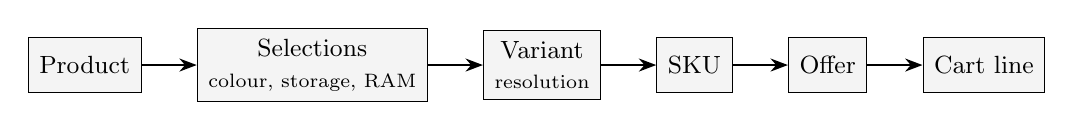
\begin{tikzpicture}[node distance=7mm]
\node[mod] (a) {Product};
\node[mod, right=of a] (b) {Selections\\\scriptsize colour, storage, RAM};
\node[mod, right=of b] (c) {Variant\\\scriptsize resolution};
\node[mod, right=of c] (d) {SKU};
\node[mod, right=of d] (e) {Offer};
\node[mod, right=of e] (f) {Cart line};
\foreach \s/\t in {a/b,b/c,c/d,d/e,e/f} \draw[arr] (\s) -- (\t);
\end{tikzpicture}
\caption{From product page to cart line. The cart stores the variant and the offer, not a product.}
\label{fig:variantflow}
\end{figure}

\paragraph{Why identity must survive.} The cart line stores the variant identifier and the offer identifier; checkout re-reads both; the order snapshots SKU, option label and seller. Two configurations of the same product are therefore two cart lines, and a line is distinguished from another by variant \emph{and} offer. The customer can see which configuration they are buying at every step, and the order still describes what was bought if the catalogue later changes. \tagimpl{} \tagtest{}

\section{Marketplace offers and the buy box}

Every variant has an implicit \emph{first-party} offer (the variant's own price and stock, sold and fulfilled by ``Cartly''). The \code{offers} table adds 608 seller offers, each with its own price, shipping charge, handling time, fulfilment mode (Cartly-fulfilled or seller-fulfilled) and stock. A cart line records which offer it came from, so the same variant from two sellers is two lines, stock is taken from the chosen offer, and a seller line carries its own shipping. \tagimpl{} \tagtest{}

The \emph{buy box} is the offer pre-selected on the page. Our rule is our own and is not Amazon's proprietary algorithm:

\begin{enumerate}
\item Consider only offers with stock; if none, show the first-party offer as unavailable.
\item Compute each offer's \emph{landed price}: price plus shipping. Offers within 2\% of the lowest landed price are contenders.
\item Among contenders prefer Cartly-fulfilled over seller-fulfilled, then the first-party offer, then shorter handling time, then lower landed price, then offer identifier.
\end{enumerate}

The final tie-break on identifier makes the outcome independent of the order in which offers happen to be read. The product page shows the selected seller, fulfilment, price, availability and delivery window, and lists the others under ``Other sellers'' with the same facts so that choosing one is an informed choice rather than noise. The seller's handling time also pushes the delivery window back (Chapter~\ref{ch:commerce}). \tagtest{} (representative tests: tie-breaks, 2\% tolerance, order independence.)

\begin{lstlisting}[caption={The contender rule, simplified from \code{catalog/offers.ts}.},label={lst:buybox}]
const lowest = Math.min(...buyable.map(landed));
const contenders = buyable.filter((o) => landed(o) <= lowest * 1.02);
// rank: Cartly-fulfilled, first-party, handling time, landed price, offer id
\end{lstlisting}

\chapter{Search, Discovery and Merchandising}
\label{ch:search}

\section{Lexical retrieval}

Search is a function of the catalogue module (\code{catalog.findProducts}) running against PostgreSQL. Each product row carries a generated full-text vector indexed with GIN; title and brand also have trigram indexes. A query goes through three progressively looser readings and stops at the first that finds anything:

\begin{enumerate}
\item every word must be the start of a word in the product (or its category name);
\item the same, but a word may also be a close misspelling of a title or brand word (trigram word similarity above a threshold of 0.5, set per transaction so it never leaks across pooled connections);
\item only half of the words (rounded up) must match, and the page then says so explicitly.
\end{enumerate}

Very common words are ignored so that nonsense such as ``this is not a product'' does not match everything, and a query made only of symbols returns nothing. Suggestions in the search box use the same machinery. \tagimpl{} \tagtest{}

\section{Structured filtering and facets}

Filters available on the results page are department, product type, brand, price range, minimum rating, in-stock only, on-sale, and the \emph{attribute facets of the chosen product type} (for example processor or refresh rate once ``Televisions'' is chosen). Facet counts ignore their own filter, so a customer can see what choosing another value would yield. Sorting (relevance, price, rating, newest) and bounded pagination are server-side; all state lives in the URL so results can be linked, reloaded and navigated with the back button. No query loads the whole catalogue into memory. \tagimpl{} \tagtest{}

\section{Hybrid retrieval: concept-based, not embedding-based}

\callout{Accuracy note}{The semantic layer is \emph{concept-based}. It does not use embeddings, a vector database, a neural model or a language model. It is a curated lexicon that maps what a query means to the product types that satisfy it.}

\paragraph{What it does.} The lexicon contains 18 concepts. Each has trigger words and an ordered list of product types, for example the intent ``keeping drinks hot or cold'' (triggers such as \emph{hot}, \emph{insulated}, \emph{commute}) maps to insulated water bottles, travel tumblers and gooseneck kettles. \code{interpretQuery} scores concepts by how many triggers match and returns up to four product types, deterministically. This lets the query \emph{``something to keep my coffee hot on my commute''}, which shares no product words with an insulated bottle, return insulated bottles and travel tumblers. \tagimpl{} \tagtest{}

\begin{figure}[H]
\centering
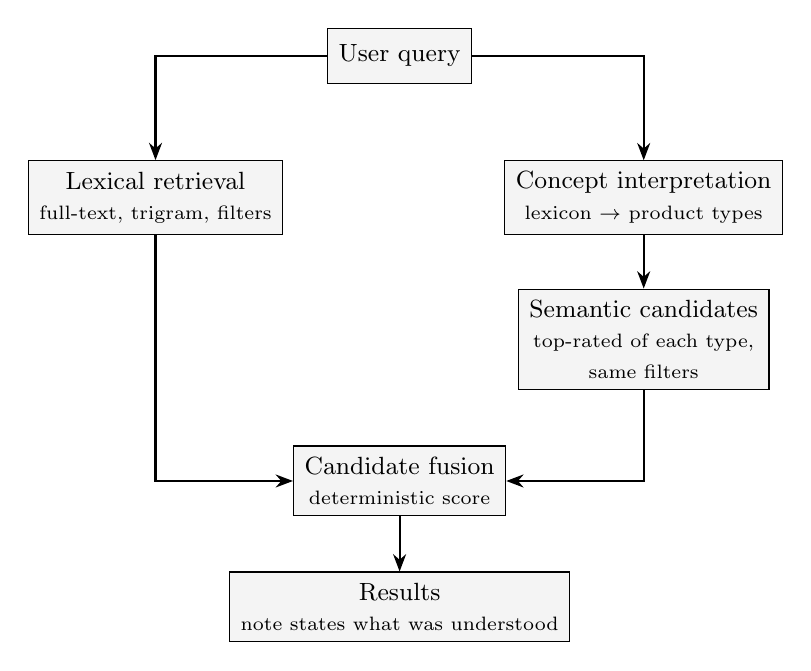
\begin{tikzpicture}
\node[mod] (q) at (3.6,0) {User query};
\node[mod] (lex) at (0.5,-1.8) {Lexical retrieval\\\scriptsize full-text, trigram, filters};
\node[mod] (con) at (6.7,-1.8) {Concept interpretation\\\scriptsize lexicon $\to$ product types};
\node[mod] (sem) at (6.7,-3.6) {Semantic candidates\\\scriptsize top-rated of each type,\\\scriptsize same filters};
\node[mod] (fuse) at (3.6,-5.4) {Candidate fusion\\\scriptsize deterministic score};
\node[mod] (res) at (3.6,-7.0) {Results\\\scriptsize note states what was understood};
\draw[arr] (q) -| (lex);
\draw[arr] (q) -| (con);
\draw[arr] (con) -- (sem);
\draw[arr] (lex) |- (fuse);
\draw[arr] (sem) |- (fuse);
\draw[arr] (fuse) -- (res);
\end{tikzpicture}
\caption{Hybrid retrieval. The lexical path always runs first and is authoritative.}
\label{fig:hybrid}
\end{figure}

\paragraph{When it runs.} The concept layer is consulted only on the first page, with relevance sorting, when no product type has been chosen, and when the words alone found fewer results than a page or only a partial match. Exact queries (``studio headphones'') are unchanged. The semantic candidates are fetched with the \emph{same} filters as the lexical ones, so price caps, brand and stock filters are respected.

\paragraph{Fusion.} Each candidate list is already in rank order. The score is
\[
\text{score} \;=\; w_{\text{lex}}\,\frac{1}{1+r_{\text{lex}}} \;+\; w_{\text{sem}}\,\frac{1}{1+r_{\text{sem}}} \;+\; w_{\text{biz}}\,\frac{\text{rating}}{5},
\]
where a product absent from a list contributes zero for that term, and ties are broken by product identifier. When the lexical match was complete the weights are $(0.6, 0.3, 0.1)$; when it was partial or empty, meaning is trusted more: $(0.25, 0.65, 0.1)$. \tagtest{} (tests assert exact scores and orderings.)

\paragraph{Fallback.} The whole semantic stage is wrapped so that any failure returns the plain lexical result. It depends on no external service.

\paragraph{Honest boundaries.} The layer understands only what the lexicon covers. During customer-perspective testing, \emph{``cheap thing for college''} returned laptops (the word ``cheap'' is not understood) and \emph{``gift for my dad''} returned home-decor items. These are weak results of exactly the kind a learned model might improve, and they are recorded here rather than hidden. The validated demonstration query is the coffee-and-commute example above. Section~\ref{sec:future} describes how this could evolve.

\section{Homepage and merchandising}

The home page is generated from data, not hand-placed. Each rail has a named source and ranking: ``today's deals'' (products with a list price above the price, best rated), ``top rated'' (in stock, by rating), ``featured'' (curated rank), ``new arrivals'' (by creation date), ``sponsored'' (active campaigns, Chapter~\ref{ch:discovery}), and, once the visitor has browsing history, ``pick up where you left off'' (recently viewed) and ``recommended for you'' (Chapter~\ref{ch:discovery}). A rail with no products renders nothing. Category tiles come from the real department facet counts. \tagimpl{}

\chapter{Pricing, Coupons and Delivery Promise}
\label{ch:commerce}

\section{The pricing flow}

Every amount the customer pays is computed on the server from the server-side cart. The browser never supplies a price, a discount or a total.

\begin{figure}[H]
\centering
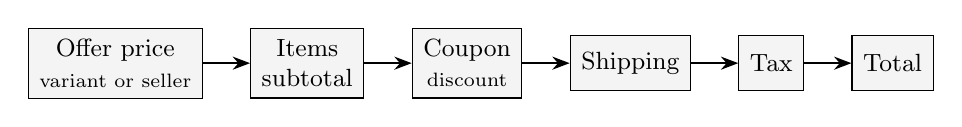
\begin{tikzpicture}[node distance=6mm]
\node[mod] (a) {Offer price\\\scriptsize variant or seller};
\node[mod, right=of a] (b) {Items\\subtotal};
\node[mod, right=of b] (c) {Coupon\\\scriptsize discount};
\node[mod, right=of c] (d) {Shipping};
\node[mod, right=of d] (e) {Tax};
\node[mod, right=of e] (f) {Total};
\foreach \s/\t in {a/b,b/c,c/d,d/e,e/f} \draw[arr] (\s) -- (\t);
\end{tikzpicture}
\caption{Order of computation (\code{checkout/internal/quote.ts}). Deals are already in the offer price as a list-price reduction.}
\label{fig:pricing}
\end{figure}

The rules are provisional demo rules, isolated in one file: first-party items ship free from a \$35.00 subtotal, otherwise \$4.99; each seller line adds the shipping that seller charges; tax is 8\% of the items \emph{after} any coupon. All arithmetic is in integer cents, with tax rounded half up. \tagimpl{} \tagtest{}

\section{Deals and coupons}

A \emph{deal} is simply an offer whose list price exceeds its price; the interface shows the original price, the price and the percentage saved. A \emph{coupon} is a row in the \code{promotions} table: a code, a kind (percent or fixed amount), a value, a minimum items subtotal and a validity window. Three demonstration codes are seeded: \code{SAVE10} (10\% off, minimum \$50.00), \code{WELCOME5} (\$5 off, minimum \$25.00) and \code{SPRING20}, which is expired on purpose so the failure path is visible.

Validation is a pure function: the code is matched case-insensitively; it must have started and not ended; the items subtotal must reach the minimum; a percentage rounds down and a discount can never exceed the subtotal. The cart stores only the \emph{code} (in a cookie); the discount is recomputed on every quote and again when checkout starts, and the order stores the code and the discount amount. A client can therefore not invent or alter a discount. The messages distinguish an unknown code, a code not yet active, an expired code and a minimum not reached, and the latter shows that code's own minimum. \tagimpl{} \tagtest{}

One limitation found during customer-perspective testing: the expired-code message does not state the expiry date.

\section{The delivery promise}

``When will it arrive'' is answered by a deterministic function (\code{catalog/delivery.ts}) that takes the current time, the fulfilment mode, the seller's handling time and, when known, the destination ZIP code.

\begin{figure}[H]
\centering
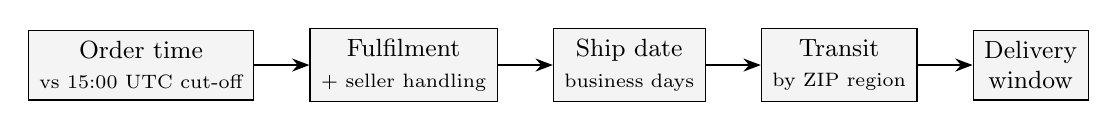
\begin{tikzpicture}[node distance=7mm]
\node[mod] (a) {Order time\\\scriptsize vs 15:00 UTC cut-off};
\node[mod, right=of a] (b) {Fulfilment\\\scriptsize + seller handling};
\node[mod, right=of b] (c) {Ship date\\\scriptsize business days};
\node[mod, right=of c] (d) {Transit\\\scriptsize by ZIP region};
\node[mod, right=of d] (e) {Delivery\\window};
\foreach \s/\t in {a/b,b/c,c/d,d/e} \draw[arr] (\s) -- (\t);
\end{tikzpicture}
\caption{Inputs to the delivery promise.}
\label{fig:delivery}
\end{figure}

The rule: orders placed before the cut-off on a weekday start processing that day, others on the next business day. Cartly-fulfilled offers ship on the processing day; seller-fulfilled offers add one business day plus one more for every 12 hours of the seller's stated handling time. Transit takes two, three or four business days depending on the first digit of the ZIP code (unknown: three), and the result is shown as a one-day window, for example ``Wed, Oct~7 -- Thu, Oct~8''. Weekends are never delivery days. For a whole cart the slowest line decides. The same function produces the text on the product page, the other-sellers list, the cart, the checkout summary and the order. \tagimpl{} \tagtest{} (four tests cover the cut-off, weekends, seller handling and destination.)

This is a simulation of a promise, not a logistics system: there are no carriers, warehouses or tracking. The separate order status timeline (placed, shipped, out for delivery, delivered) runs on a compressed demo clock, and the report does not claim the two represent the same real-world process.

\chapter{Inventory Consistency, Checkout and Payments}
\label{ch:inventory}

\section{Why stock needs reservations}

A naive checkout reads the stock, charges the card and decrements the stock at the end. Between the read and the write another customer can do the same, and the last unit is sold twice. Charging first and decrementing later is worse, because the failure appears after the money moved. This project instead \emph{reserves} stock when checkout starts, converts the reservation into a sale only when payment is confirmed, and releases it on failure, expiry or cancellation.

\section{The reservation model}

Table \code{stock\_reservations} holds one row per order, variant and offer with a quantity, an expiry time and a status: \emph{held}, \emph{committed} or \emph{released}. A unique constraint on (order, variant, offer) makes reserving idempotent. A hold lasts 15 minutes. Expiry is evaluated lazily: a hold whose time has passed is simply ignored when availability is computed, so no background job is required. \tagimpl{}

To reserve, the module locks the stock row for the variant (or the offer, for seller lines), counts the unexpired holds of \emph{other} orders, and refuses if the remaining stock is smaller than the request. Lines are processed in a fixed order to avoid deadlocks, and all lines succeed or none do. Because the stock row is locked first, two customers racing for the final unit are serialised by the database: the second one sees the first one's hold and fails. Commit re-checks the same condition, so a hold that expired and was taken by someone else cannot be committed. \tagtest{}

\begin{figure}[H]
\centering
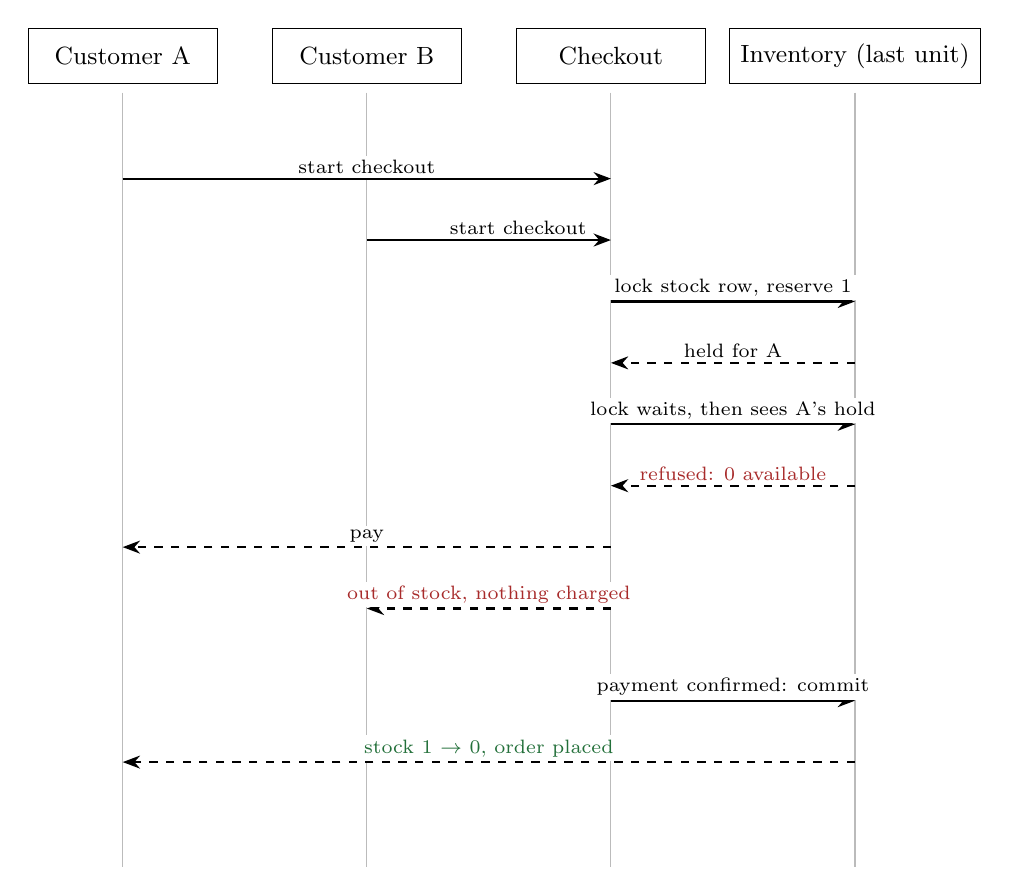
\begin{tikzpicture}[x=3.1cm, y=-0.78cm, font=\scriptsize]
\foreach \x/\n in {0/Customer A, 1/Customer B, 2/Checkout, 3/Inventory (last unit)} {
  \node[box, minimum width=2.4cm] (h\x) at (\x,0) {\n};
  \draw[rule] (\x,0.6) -- (\x,13.2);
}
\draw[arr] (0,2) -- node[lbl,above]{start checkout} (2,2);
\draw[arr] (1,3) -- node[lbl,above, pos=0.62]{start checkout} (2,3);
\draw[arr] (2,4) -- node[lbl,above]{lock stock row, reserve 1} (3,4);
\draw[darr] (3,5) -- node[lbl,above]{held for A} (2,5);
\draw[arr] (2,6) -- node[lbl,above]{lock waits, then sees A's hold} (3,6);
\draw[darr] (3,7) -- node[lbl,above, text=risk]{refused: 0 available} (2,7);
\draw[darr] (2,8) -- node[lbl,above]{pay} (0,8);
\draw[darr] (2,9) -- node[lbl,above, text=risk]{out of stock, nothing charged} (1,9);
\draw[arr] (2,10.5) -- node[lbl,above]{payment confirmed: commit} (3,10.5);
\draw[darr] (3,11.5) -- node[lbl,above, text=ok]{stock 1 $\to$ 0, order placed} (0,11.5);
\end{tikzpicture}
\caption{Two customers, one unit. The database lock serialises the reservations; only A can proceed to payment.}
\label{fig:race}
\end{figure}

This is a single-database transactional design. It is correct for one PostgreSQL primary and would need a different mechanism (for example a dedicated inventory service) at multi-region scale; Chapter~\ref{ch:decisions} says so.

\textbf{Evidence.} The module-level test starts both checkouts concurrently against the real database and asserts that exactly one succeeds; an end-to-end test drives two separate browser sessions through the checkout form at the same moment and asserts that exactly one sees ``Order placed'' and the other a sold-out message with nothing charged. Further tests cover expiry (a freed unit becomes buyable by the other customer), release on cancellation, and a late payment after expiry (the order is honoured if the unit is still free, otherwise cancelled and refunded). \tagtest{}

\section{Three separate states}

The central design rule of the payment system is that \emph{inventory, payment and order are three state machines that never share a field}. The order is not ``paid'' because a button was clicked; it is placed because the payment record says succeeded, and the stock is sold at that same moment.

\begin{figure}[H]
\centering
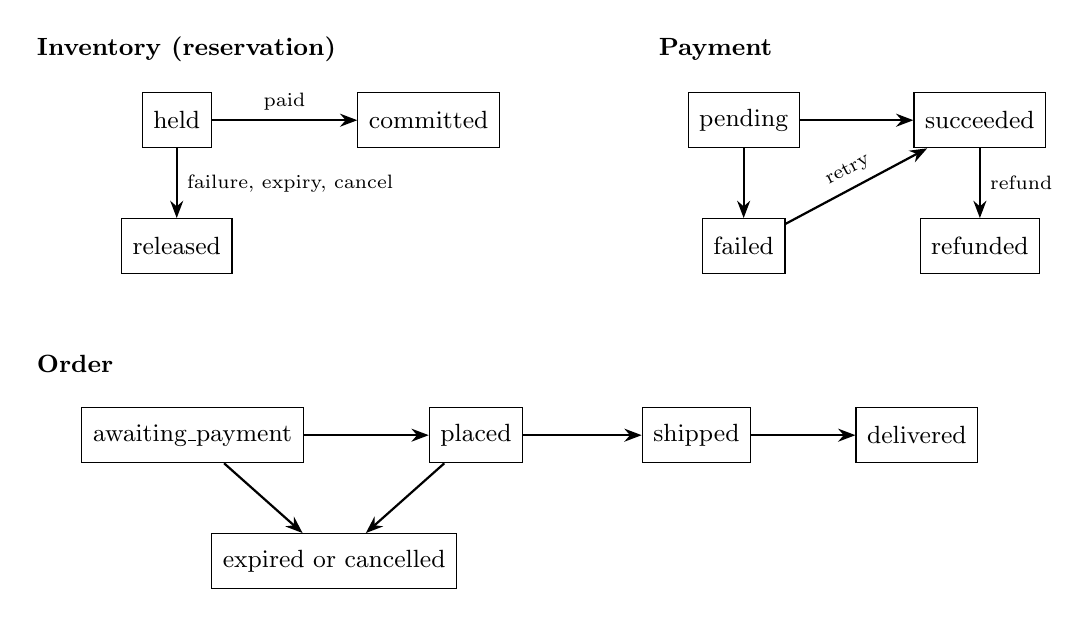
\begin{tikzpicture}[font=\scriptsize]
\node[font=\small\bfseries, anchor=west] at (-0.5,0.9) {Inventory (reservation)};
\node[box] (h) at (1.4,0) {held};
\node[box] (c) at (4.6,0) {committed};
\node[box] (r) at (1.4,-1.6) {released};
\draw[arr] (h) -- node[above]{paid} (c);
\draw[arr] (h) -- node[right]{failure, expiry, cancel} (r);

\node[font=\small\bfseries, anchor=west] at (7.4,0.9) {Payment};
\node[box] (p) at (8.6,0) {pending};
\node[box] (s) at (11.6,0) {succeeded};
\node[box] (f) at (8.6,-1.6) {failed};
\node[box] (rf) at (11.6,-1.6) {refunded};
\draw[arr] (p) -- (s);
\draw[arr] (p) -- (f);
\draw[arr] (f) -- node[above, sloped]{retry} (s);
\draw[arr] (s) -- node[right]{refund} (rf);

\node[font=\small\bfseries, anchor=west] at (-0.5,-3.1) {Order};
\node[box] (a) at (1.6,-4.0) {awaiting\_payment};
\node[box] (pl) at (5.2,-4.0) {placed};
\node[box] (sh) at (8.0,-4.0) {shipped};
\node[box] (dl) at (10.8,-4.0) {delivered};
\node[box] (ex) at (3.4,-5.6) {expired or cancelled};
\draw[arr] (a) -- (pl);
\draw[arr] (pl) -- (sh);
\draw[arr] (sh) -- (dl);
\draw[arr] (a) -- (ex);
\draw[arr] (pl) -- (ex);
\end{tikzpicture}
\caption{The three state machines (scaled to fit). The order also carries a separate refund status (pending, refunded, failed). Shipped and delivered are derived from time, not stored.}
\label{fig:states}
\end{figure}

\section{Two-phase checkout}

\paragraph{Phase 1: start checkout} (one database transaction). Validate the address; take an advisory lock on the customer and idempotency key; re-read the server cart and price it, including any coupon; abandon the customer's other unpaid orders; create the order in the \emph{awaiting payment} state with purchase-time snapshots; reserve stock. Then, outside the transaction, ask the payment provider to create the payment. Starting again with the same key returns the same order; if the cart has changed meanwhile it is refused with a clear message rather than silently repriced. The cart is \emph{not} cleared yet. \tagimpl{} \tagtest{}

\paragraph{Phase 2: payment event} (one transaction). A provider event is recorded and de-duplicated, the pure state function updates the payment, and only if the payment is now \emph{succeeded} does checkout commit the reservations, mark the order paid (this starts the fulfilment clock), and clear the cart. If the order was cancelled meanwhile, or the held units can no longer be committed, the order is cancelled and the money is refunded instead of being double-sold.

\section{Payment provider boundary}

Checkout depends on a \code{PaymentProvider} interface: create a payment, retrieve it, cancel it, refund it, verify a webhook, and (demonstration provider only) accept card details. Nothing in the interface returns ``the customer paid''; success can arrive only as a verified event or a server-side retrieval. Two implementations exist: a demonstration provider that simulates a bank (used locally and in tests) and a Stripe implementation in test mode. The application selects Stripe when a Stripe secret key is configured. \tagimpl{}

\subsection{Stripe test mode}

On the server, the order total is used to create a PaymentIntent with the order identifier in its metadata and an idempotency key. The browser receives only the client secret and the publishable key and renders Stripe's Payment Element; card data never touches the application server. After confirmation Stripe redirects the customer to the order page, but that redirect is not trusted. The order is placed by one of two server-side paths:

\begin{enumerate}
\item \textbf{Signed webhook.} A route handler reads the \emph{raw} request body, verifies the signature with the webhook secret, and maps recognised events (payment succeeded, failed, processing, requires action, canceled, charge refunded) into the application's own event type. Unrecognised events and events for unknown payments are acknowledged without effect; a bad signature is rejected; an internal error returns a failure so Stripe retries.
\item \textbf{Server-side retrieval.} The payment and confirmation pages ask Stripe for the PaymentIntent and handle the answer exactly like an event, so a delayed or missing webhook cannot strand a paid order.
\end{enumerate}

\paragraph{Idempotency and ordering.} Events are recorded by provider event identifier, so a replay changes nothing. A pure state function accepts success from any open state, ignores events older than the last applied one, and allows refunds only after success; therefore a late ``failed'' event cannot undo a success. A refund row is written as pending \emph{before} the provider is called, its identifier is the provider's idempotency key, and the payment counts as refunded only when the provider says the refund succeeded. A failed refund is shown as failed and can be retried; the interface never claims a refund that has not happened.

\begin{lstlisting}[caption={Rule from the payment state function, simplified.},label={lst:paystate}]
// success wins from any non-final state; other changes only while open and not older
if (event.type === "payment.succeeded" && !isFinal(state)) return succeeded;
if (isOlder(event, state.lastEventAt)) return unchanged;
\end{lstlisting}

\paragraph{Evidence and its limits.} The webhook path is covered by five tests that use the real Stripe signature verification with generated signatures (replay, tampered body, missing signature, out-of-order events, unknown payment, refund after cancellation); the state machine and checkout flow are covered by the payment-flow tests. \tagtest{} A completed card payment against the live Stripe API from this repository was \emph{not} performed or recorded; the key-gated browser test for it exists but was not run. \tagunver{} In production the checkout button reads ``Continue to payment'', which indicates a Stripe key is configured, but successful settlement is unconfirmed.

\section{Cancellation and refunds}

Cancellation is allowed while an order is awaiting payment (the hold is released and the payment cancelled) and, for a paid order, only during the first minutes while it is still ``placed''. A paid cancellation restocks the units in the same transaction, then requests a refund from the provider and records the outcome separately from the order status.

\chapter{Recommendations, Sponsored Placements and Reviews}
\label{ch:discovery}

\section{Recently viewed and personalisation}

Every product page view is recorded against the visitor (signed-in user, or an anonymous browser identifier) in \code{product\_views}, one row per visitor and product, newest first. The anonymous identifier lives in its own cookie, separate from the cart's guest token: an early version recorded views with the cart token and could race with cart creation, so the two were separated. On sign-in the anonymous history is merged into the account. The home page uses it to show ``Pick up where you left off'' and ``Recommended for you''; with no history, those rails are simply absent and the generic rails remain. \tagimpl{} \tagtest{}

\section{Deterministic recommendations}

Recommendations are a transparent weighted sum computed from a bounded candidate pool (the best-rated products of each seed's type and category). For a seed product and a candidate:

\begin{table}[H]
\centering
\caption{Recommendation signals (\code{discovery/score.ts}).}
\label{tab:reco}
\small
\begin{tabular}{@{}lr@{}}
\toprule
Signal & Contribution \\
\midrule
Same product type & $+4$ \\
Same category (different type) & $+2$ \\
Same brand & $+2$ \\
Shared attribute values & $+0.5$ each, at most 3 \\
Price proximity (log scale) & $0$ to $+2$ \\
Rating & $0$ to $+1.5$ \\
Popularity (rating count, capped at 1,000) & $0$ to $+1$ \\
On sale & $+0.75$ \\
\bottomrule
\end{tabular}
\end{table}

With several seeds (the last three viewed products) each seed's similarity is divided by its recency rank, so the most recent view counts most. Seeds and out-of-stock products are never recommended, and ties break on product identifier. The same function powers ``Related products'' on a product page (one seed) and ``Recommended for you'' (up to three seeds). \tagimpl{} \tagtest{}

We chose a transparent rule over a trained model because the time box allowed no data to train on, because a rule can be explained to a customer and a reviewer, because it is reproducible (the same inputs always give the same page, which makes it testable), and because it needs no infrastructure. It is not machine learning and the report does not call it that.

\section{Sponsored placements}

A sponsored campaign is a row in \code{sponsored\_campaigns}: a product, a placement (search or home), keywords, a bid, a budget and a date window. The service returns active campaigns with budget remaining, ordered by bid (ties by identifier). For search placements the campaign's keywords must match the query; products already in the organic results are excluded so a product never appears twice.

The crucial property is separation: sponsored products are returned by a separate call and rendered in their own block labelled ``Sponsored''; they never enter, reorder or alter the organic ranking, which a test asserts by comparing organic results before and after. A sponsored product that is out of stock is not shown. This is an observable simulation of marketplace advertising, not an ad auction: there is no pricing mechanism, spend accounting or relevance model. \tagimpl{} \tagtest{}

\section{Reviews and trust}

A review stores a product, an optional variant, an author, a rating from one to five, a title, a body, a ``verified'' flag and a timestamp. Three properties matter.

\begin{itemize}
\item \textbf{Verified means something.} The flag is set only by the server, and only when the signed-in user has a \emph{delivered} order containing a variant of that product; a client cannot claim it. A user may review a product once, and an order that is merely placed does not qualify. \tagtest{}
\item \textbf{Aggregates are real.} The displayed rating and count of a product are recomputed from its review rows (at seeding, and after each new review), and the page shows the average, the count, a five-bar distribution and the review text with a verified badge.
\item \textbf{Seeded data is labelled honestly.} The catalogue is seeded with two to eight invented reviews per product written from templates and a seeded random generator, with some flagged verified. These flags are synthetic data, not outcomes of the eligibility rule. The demonstration account (credentials documented in the repository for demo use) has three delivered orders so that the real rule can be shown live.
\end{itemize}

Verified reviews are more meaningful than arbitrary star averages because they connect an opinion to a completed transaction. In this project that connection is real for new reviews and simulated for seeded ones, and the report keeps that distinction.

\chapter{Customer Experience and Performance}
\label{ch:ux}

\section{Customer-facing decisions}

The interface follows a restrained monochrome direction (white, black and neutral greys, one typeface, black primary actions, no gradients or decorative shadows), recorded as a design decision after an earlier warmer direction was rejected. Beyond appearance, the useful question was what a customer who has never seen the system will expect, misunderstand and be frustrated by. Decisions that followed:

\begin{itemize}
\item \textbf{Identity of what is being bought.} Variant labels, SKU and seller appear on the product page, in the cart and on the order, so the customer can see which configuration and from whom.
\item \textbf{The cart survives.} The cart is stored on the server against the signed-in user or a guest cookie, so reloads and navigation do not lose it; a guest cart merges into the account on sign-in. Removing an item offers an undo. Quantity controls are clamped to available stock with an explanation, rather than failing at checkout.
\item \textbf{Guest checkout is open.} Accounts add history; they do not gate purchase.
\item \textbf{Coupon feedback.} Invalid, expired and under-minimum codes each get a specific message.
\item \textbf{Delivery and seller visibility.} The delivery window and seller are shown at the purchase decision, in the cart and at checkout, not only after ordering.
\item \textbf{Empty and failure states.} An empty cart, a search with no results (with department links), an expired checkout hold, a declined payment and a sold-out item each say what happened and what to do next. A declined payment keeps the cart and the typed address.
\item \textbf{Mobile.} The product page gets a sticky purchase bar when the primary action scrolls away; filters open in a deliberate sheet; automated checks verify that key pages do not overflow horizontally on a phone viewport.
\item \textbf{Accessibility.} Semantic structure, labelled form fields, announced status and error messages, visible focus and touch-sized targets were part of the design rules; a browser audit at widths from 320 to 1440 pixels was recorded in the project documents.
\item \textbf{No manufactured urgency.} Stock messages reflect real stock.
\end{itemize}

Customer-perspective testing of the deployed site found three small defects, two of which were fixed before this report: a footer that still said payments were simulated while Stripe was active, and a coupon message that showed the wrong minimum spend. The third (weak results for some vague meaning queries) is described in Chapter~\ref{ch:search}. Several customer paths were \emph{not} tested manually in this review: back and forward navigation through checkout, quantity extremes, a sell-out during checkout, and the full mobile purchase flow. Some are covered by automated tests; the rest are listed in the limitations.

\section{Performance and scale}

The architecture avoids the usual early mistakes rather than claiming scale it has not proven.

\begin{itemize}
\item Search and filtering run in indexed SQL; pages never load the catalogue. Result pages are bounded and paginated.
\item Indexes exist for full-text and trigram search, brand, category, type, attributes (GIN), variants by product, reservations by unit, orders by owner, offers by variant, order items by order and product rating ordering.
\item Facets and result pages issue a fixed number of queries independent of result size.
\item Product pictures use lazy loading except for the first row, and the purchase and checkout screens are server-rendered.
\item Writes that must be consistent (checkout start, payment confirmation, cancellation) are single transactions.
\end{itemize}

\paragraph{Measurements recorded in the repository.} Early in the work the search approach was measured on PGlite before committing to PostgreSQL search. A throwaway benchmark on synthetic rows found that loading and joining the whole catalogue per query cost 63~ms at 3,000 products and 269~ms at 12,000 (and three such queries on the home page), while an indexed full-text query stayed at 1.4~ms and 3.9~ms and a trigram typo query at 2.6~ms and 8.5~ms at those sizes. After the 2,400-product build, warm requests on a production build with in-memory PGlite on a loaded laptop measured about 85--120~ms for the home page, 80--135~ms for a results page, 50--70~ms for a deep category page, about 0.2~s for a typo query and 30--50~ms for a product page. These were measured on PGlite (PostgreSQL compiled to WebAssembly), not on the deployed database, and the project documents state that they must be re-measured there. No load test was run.

\paragraph{Current implementation versus production scale.} At Amazon's actual scale the catalogue, search, inventory, pricing and recommendation systems are separate services with their own data stores and teams. This project is one program and one primary database. It demonstrates correct behaviour at a few thousand products, not capacity at hundreds of millions; Chapter~\ref{ch:decisions} describes what would change.

\chapter{Testing, Security and Deployment}
\label{ch:quality}

\section{Testing and quality engineering}

\begin{table}[H]
\centering
\caption{Test layers and results at the time of writing.}
\label{tab:tests}
\small
\begin{tabularx}{\linewidth}{@{}p{2.6cm}XXp{2.4cm}@{}}
\toprule
Layer & Purpose & Coverage & Result \\
\midrule
Pure unit tests & Rules with no I/O & Buy box, delivery promise, coupons, recommendation scoring, payment state function, variant resolution, concept lexicon, fusion score & Pass \\
Integration tests (real PostgreSQL engine) & Module behaviour through public interfaces & Reservations and last-unit race, two-phase checkout, payment flow, webhook signatures, refunds, reviews eligibility, recently viewed, sponsored placement, hybrid search, seeding & 131 tests in 26 files pass \\
End-to-end (Playwright) & Real browser against a production build, fresh in-memory database & 12 scenarios on a desktop and a phone (Pixel 7) viewport: discovery with typo recovery, purchase, variants, offers, structured search, lifecycle and cancellation, declined-card recovery, guest-to-account, overflow check, two-shopper race & Last full run: 18 run and passed, 6 skipped by design; later subset runs passed \\
Stripe browser test & Real Payment Element, test card and decline & Two scenarios & Skipped without keys; \tagunver{} \\
Static checks & Types and boundaries & TypeScript strict; ESLint including the module-boundary rule & Clean \\
\bottomrule
\end{tabularx}
\end{table}

Tests carry stable identifiers (T1 to T132) that the decision log refers to. Representative examples: T104 starts two checkouts for the last unit concurrently and asserts that exactly one succeeds; T100 delivers a payment success after the hold expired, once when the unit is free (order placed) and once when another customer bought it (order cancelled and refunded, never double-sold); T97 and T98 show a declined payment keeping the order and hold, and a retry succeeding; T105--T109 replay, tamper with and reorder signed webhook events; T119--T121 and T132 cover coupon arithmetic, trust boundary and messages; T122 checks the buy-box tolerance and order independence; T114--T118 check that recommendations are deterministic and exclude the seed and out-of-stock items; T123 checks the verified-review rule end to end; T125 shows sponsored placement leaves organic results unchanged; T127--T131 cover the concept lexicon, fusion and fallback.

A CI workflow (lint, type check, unit and integration tests; no secrets needed) is in the repository but its first run on GitHub was not observed; the browser tests are run locally because they use the installed Chrome. One tooling lesson from development: running a development server and a production build in the same working directory corrupted an end-to-end run; it was diagnosed and avoided.

\section{Security and trust boundaries}

Only measures that exist in the code are listed. This is a demonstration project and no penetration test was performed.

\begin{itemize}
\item \textbf{Server-side money.} Prices, discounts, shipping, tax, totals and the payment amount are computed on the server from server-held state. The client sends a coupon \emph{code} and quantities, nothing monetary.
\item \textbf{Payment authority.} The order is placed only from a signature-verified Stripe webhook over the raw request body, or from a server-side retrieval of the PaymentIntent. The browser redirect and the client library's result are not trusted.
\item \textbf{Secrets.} Database URL and Stripe keys exist only as environment variables; only the Stripe publishable key reaches the browser. A scan of tracked files found no keys or connection strings (only fake values in a unit test). Raw reference captures that could contain a real person's session data are excluded from the repository by ignore rules.
\item \textbf{Authentication.} Passwords are hashed with scrypt and a per-user salt and compared in constant time; a dummy hash equalises timing for unknown emails. Session tokens are random, stored only as hashes, and sent in HTTP-only, SameSite cookies marked secure in production; sessions expire after 30 days.
\item \textbf{Access control.} Orders and carts are scoped to their owner key; fetching another customer's order identifier returns nothing. Reviews require a delivered order.
\item \textbf{Input handling.} Inputs are parsed with Zod at the boundary; queries use parameterised SQL through the ORM; free-text search input is normalised and bounded.
\item \textbf{Idempotency and replay.} Duplicate form submissions, duplicate webhooks and repeated refunds are safe by construction (Chapter~\ref{ch:inventory}).
\end{itemize}

Not implemented: rate limiting, CSRF tokens beyond the framework's server-action protections, bot protection, fraud screening and audit logging.

\section{Deployment}

\begin{figure}[H]
\centering
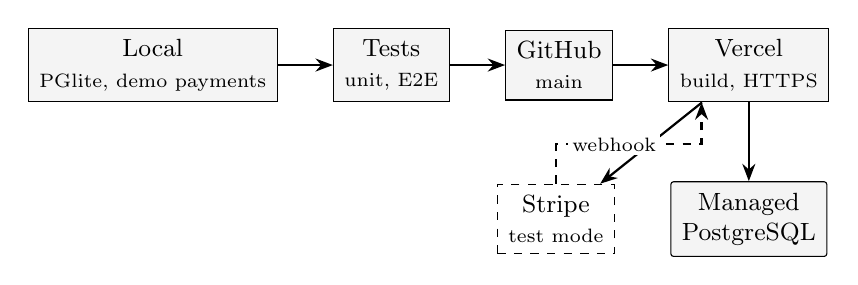
\begin{tikzpicture}[node distance=7mm]
\node[mod] (dev) {Local\\\scriptsize PGlite, demo payments};
\node[mod, right=of dev] (test) {Tests\\\scriptsize unit, E2E};
\node[mod, right=of test] (gh) {GitHub\\\scriptsize main};
\node[mod, right=of gh] (vc) {Vercel\\\scriptsize build, HTTPS};
\node[store, below=10mm of vc] (pg) {Managed\\PostgreSQL};
\node[ext, left=of pg] (st) {Stripe\\\scriptsize test mode};
\foreach \s/\t in {dev/test,test/gh,gh/vc} \draw[arr] (\s) -- (\t);
\draw[arr] (vc) -- (pg);
\draw[arr] (vc) -- (st);
\draw[darr] (st.north) -- ++(0,5mm) -| node[lbl, pos=0.2]{webhook} ([xshift=-6mm]vc.south);
\end{tikzpicture}
\caption{Path from development to production.}
\label{fig:deploy}
\end{figure}

The same SQL runs everywhere: PGlite locally and in tests, a pooled PostgreSQL connection in production, selected by whether \code{DATABASE\_URL} is set. Migrations and seeding are not run on requests; the Vercel build command applies migrations and seeds an empty database (idempotently) before building. The deployment documents choose Neon as the managed PostgreSQL host; the repository cannot confirm which host the live deployment uses. GitHub records production deployments of the final commits as successful and the site serves over HTTPS. The Stripe webhook endpoint is \code{/api/webhooks/stripe}; an unsigned request is rejected with HTTP 400, which was checked against the live site. Webhook delivery from Stripe to the live endpoint and the full payment were not verified. \tagunver{}

\chapter{Engineering Decisions, Limits and Future Architecture}
\label{ch:decisions}

\section{Decisions and tradeoffs}

\begin{table}[H]
\centering
\caption{Principal decisions (numbers refer to the repository's decision log).}
\label{tab:decisions}
\footnotesize
\begin{tabularx}{\linewidth}{@{}p{2.7cm}XXX@{}}
\toprule
Decision & Alternatives considered & Why chosen & Tradeoff \\
\midrule
PostgreSQL for search (D23) & Dedicated search engine; keeping the earlier in-memory search & Benchmarks showed in-memory scanning degrading by 3,000 products while indexed SQL stayed in milliseconds; one system to operate & Weaker relevance tuning; no learned ranking \\
Concept-based hybrid retrieval (D32) & Embeddings with pgvector or a hosted model & No installed model, no new paid service or secret, deterministic and testable, graceful fallback & Understands only the lexicon; some vague queries return weak results \\
Deterministic recommendations (D30) & Trained model & No training data in the time box; explainable and reproducible & Cannot learn from behaviour \\
Modular monolith (modules document) & Microservices & One deployable unit; boundaries enforced by lint; fits one developer & Boundaries are social plus tooling, not network \\
Provider interface for payments (D28) & Calling Stripe directly & Demo provider for tests; webhook and retrieval share one event handler & An extra abstraction to maintain \\
Reservation-based stock (D27) & Decrement at payment; optimistic retry & Prevents selling twice and charging for unavailable stock & Holds stock for 15 minutes from abandoned checkouts \\
Synthetic catalogue (D23) & Scraped or licensed product data & No data rights; deterministic and reproducible & Product data is obviously artificial \\
Implicit first-party offer (D26) & Every variant as explicit offers & No migration of existing cart and checkout; seller offers are additive & Two code paths for the first-party and seller cases \\
Derived order timeline (D24) & Stored statuses with a job runner & No scheduler needed; consistent with the clock & Time compressed for demonstration \\
Guest checkout open (D22) & Required accounts & Fewer abandoned purchases & Accounts add history, not security of the purchase \\
\bottomrule
\end{tabularx}
\end{table}

\section{What was deliberately not built}

\begin{itemize}
\item \textbf{Distributed search and learned ranking.} The catalogue is small and the ranking is rules; a dedicated engine would add infrastructure without a visible gain in the time box.
\item \textbf{Machine-learned recommendation and an ad auction.} No behavioural data or traffic exists to learn from; the observable behaviour (separation, labelling, determinism) was the point.
\item \textbf{Warehouse management and a real logistics network.} Inventory is a count per variant or offer; delivery is a deterministic simulation.
\item \textbf{Seller operations.} No seller portal, onboarding, payouts or seller ratings.
\item \textbf{Live payments, saved cards and fraud detection.} Stripe test mode only; card data never touches the server.
\item \textbf{Large-scale personalisation infrastructure.} Personalisation is a per-visitor view history.
\item \textbf{Reviews beyond the basics.} No helpful votes, images or moderation.
\item \textbf{Email, returns, internationalisation, tax by jurisdiction.} A single country and provisional tax and shipping rules.
\end{itemize}

Each was deferred because it either needed infrastructure or data that the time box could not supply or would not change what a reviewer could verify about the system's correctness.

\section{Limitations}

\paragraph{Product.} The catalogue, sellers, reviews and campaigns are synthetic and the pictures are generated illustrations. Some vague meaning queries return weak results. The expired-coupon message has no date. Taxes and shipping are demo rules.

\paragraph{Infrastructure.} One application and one primary database; no cache layer, queue, search service, observability stack or rate limiting. Reservation expiry is lazy, which is correct for availability but means abandoned holds are not actively cleaned.

\paragraph{Scale.} Measured behaviour is for a few thousand products on PGlite and a managed database of modest size; no load test was run and the recorded timings were not repeated on the deployed database.

\paragraph{Validation.} A completed live Stripe test payment and webhook delivery were not confirmed from the repository; the Stripe browser tests were skipped for lack of keys; the first CI run on GitHub was not observed; several customer paths (back-navigation through checkout, mid-checkout sell-out, full mobile purchase) were not manually verified in a final pass.

\section{Future architecture}\label{sec:future}

\callout{Label}{This section describes possible evolution. None of it exists in the repository.}

If the prototype became a product, the natural seams are already the module boundaries:

\begin{itemize}
\item \textbf{Catalogue and search services.} Move catalogue ingestion and indexing behind a service with a search engine for relevance and facets; keep PostgreSQL as the source of truth. A learned retriever (embeddings) could replace the concept lexicon, with the lexical path retained as the fallback exactly as today.
\item \textbf{Inventory service.} Extract reservations into a service with per-location stock and expiry workers, preserving the held, committed, released lifecycle.
\item \textbf{Payments and order management.} Keep the provider interface; add live-mode controls, asynchronous reconciliation against the provider and a returns and refund workflow.
\item \textbf{Fulfilment and delivery.} Replace the deterministic promise with carrier and warehouse data, keeping the same function signature as the contract.
\item \textbf{Recommendation and ads platforms.} Train ranking from behavioural events, run experiments, and add an auction with budgets and reporting, retaining the rule that sponsored content is separate and labelled.
\item \textbf{Seller platform, analytics and experimentation.} Seller onboarding and ratings; event pipelines and A/B testing.
\end{itemize}

\chapter{Final Engineering Takeaways}
\label{ch:conclusion}

\begin{itemize}
\item \textbf{The frontend is the visible surface.} The pages that look like a shop are the output of a catalogue model, offers, reservations, a payment lifecycle and ranking rules. Most of the effort, and nearly all of the risk, sat below the interface.
\item \textbf{Domain modelling pays for itself.} Separating product, variant and offer made variants, sellers, the buy box, the cart and order snapshots fall out of one idea rather than becoming special cases.
\item \textbf{State transitions need an owner.} Treating inventory, payment and order as three machines, and letting only verified events move the payment machine, removed a class of bugs (double sale, order without payment, refund claimed but not made) by construction.
\item \textbf{Customer experience depends on backend correctness.} Clear messages for an expired hold, an under-minimum coupon or a declined card are only possible because the backend returns distinct, typed outcomes.
\item \textbf{Deterministic systems are often the right choice under a deadline.} Rules for ranking, recommendations, delivery and concept search are explainable, reproducible and testable; their limits are known and were written down instead of hidden.
\item \textbf{Scope management is an engineering skill.} What was left out (Chapter~\ref{ch:decisions}) was chosen deliberately, and the order of work protected the purchase path first.
\item \textbf{Reliability beats feature count.} A smaller set of features, each with tests and an honest statement of what is and is not verified, is more useful than a longer list that cannot be trusted. The unverified items in this report, chiefly a completed live Stripe payment, are the most important follow-up work.
\end{itemize}

\end{document}
